\documentclass[11pt,letterpaper]{article}
\usepackage[margin=.65in,top=.78in,bottom=.65in]{geometry}
\usepackage[T1]{fontenc}
\usepackage{lmodern,tikz,array,fancyhdr}
\usetikzlibrary{arrows.meta}
\renewcommand{\familydefault}{\sfdefault}
\pagestyle{fancy}\fancyhf{}
\fancyhead[L]{\small Week 73 / The gentlest stretch / Grades 4--5}
\fancyfoot[L]{\small Bellingham Math Circle / Week 73 / GGT73-S-draft}
\fancyfoot[R]{\small\thepage}
\renewcommand{\headrulewidth}{0pt}\renewcommand{\footrulewidth}{0pt}
\setlength{\parindent}{0pt}\setlength{\parskip}{8pt}
\newcommand{\problem}[2]{\textbf{Problem #1:} #2\par}
\newcommand{\answerline}{\par\vspace{.32in}\hrule height .25pt}
\newcommand{\fanboard}{\begin{center}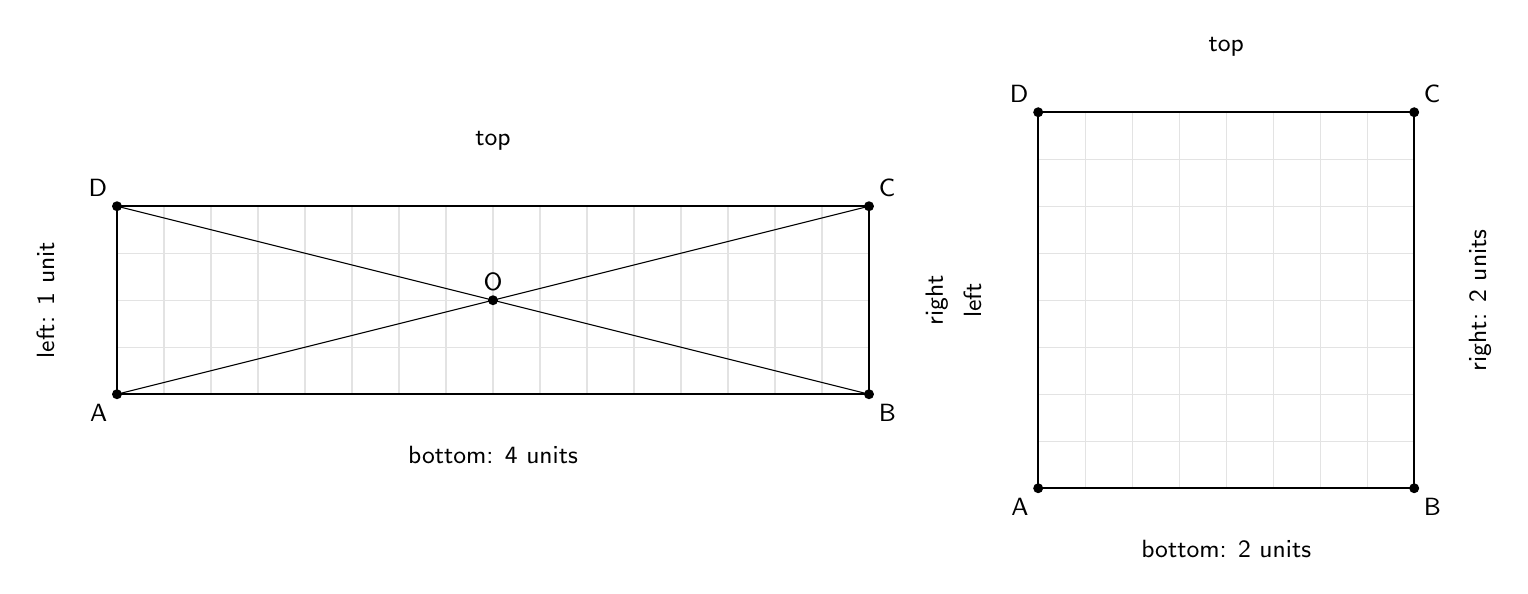
\begin{tikzpicture}[x=.94in,y=.94in,font=\small]
\draw[step=.25,gray!22] (0,.5) grid (4,1.5);
\draw[thick] (0,.5) rectangle (4,1.5);
\foreach \x/\y/\name/\pos in {0/.5/A/below left,4/.5/B/below right,4/1.5/C/above right,0/1.5/D/above left}{\fill (\x,\y) circle (1.8pt);\node[\pos] at(\x,\y){\name};\draw (\x,\y)--(2,1);}
\fill (2,1) circle (1.8pt);\node[above] at(2,1){O};
\node at (2,.18) {bottom: 4 units};\node at(2,1.85){top};\node[rotate=90] at(-.38,1){left: 1 unit};\node[rotate=90] at(4.36,1){right};
\draw[step=.25,gray!22,xshift=4.9in*.94] (0,0) grid (2,2);
\begin{scope}[shift={(4.9,0)}]
\draw[thick] (0,0) rectangle(2,2);
\foreach \x/\y/\name/\pos in {0/0/A/below left,2/0/B/below right,2/2/C/above right,0/2/D/above left}{\fill(\x,\y)circle(1.8pt);\node[\pos]at(\x,\y){\name};}
\node at(1,-.32){bottom: 2 units};\node at(1,2.35){top};\node[rotate=90]at(-.35,1){left};\node[rotate=90]at(2.35,1){right: 2 units};
\end{scope}
\end{tikzpicture}\end{center}}
\begin{document}
Use paper dots, a ruler and strips of paper to compare straight-line distances.
Match dots with the same letters. A pair's stretch is its new distance divided by its old distance.
\begin{center}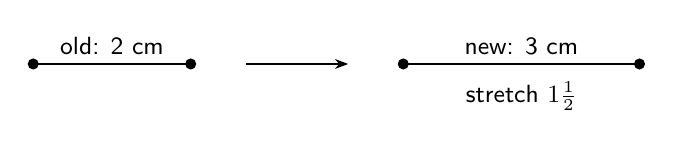
\begin{tikzpicture}[x=1cm,y=1cm,font=\small,>=Stealth]
\draw[thick] (0,0)--(2,0);\fill(0,0)circle(2pt);\fill(2,0)circle(2pt);
\node[above]at(1,0){old: 2 cm};
\draw[->](2.7,0)--(4,0);
\draw[thick](4.7,0)--(7.7,0);\fill(4.7,0)circle(2pt);\fill(7.7,0)circle(2pt);
\node[above]at(6.2,0){new: 3 cm};\node[below]at(6.2,-.1){stretch $1\frac12$};
\end{tikzpicture}\end{center}
\problem{1}{Place O inside the square, not on an edge. Your partner chooses pairs from A, B, C, D and O and measures their stretch. Your score is the largest stretch found. Try to make the score as small as possible. Swap jobs and try different positions for O.}
\fanboard
\vspace{.12in}
\begin{tabular}{@{}p{.39\linewidth}p{.26\linewidth}p{.23\linewidth}@{}}
O's position & Pair tested & Stretch\\\hline
 & & \\[.35in]\hline
 & & \\[.35in]\hline
 & & \\[.35in]\hline
 & & \\[.35in]\hline
\end{tabular}\par
\newpage
\problem{2}{Join O to all four corners in the square. Each old triangle moves evenly onto its matching new triangle: straight segments stay straight, and halfway points stay halfway. Your partner places O. Add halfway dots on triangle edges and hunt for a pair that stretches more than any pair of the original five dots. Swap jobs. Which positions for O survive every test?}
\begin{center}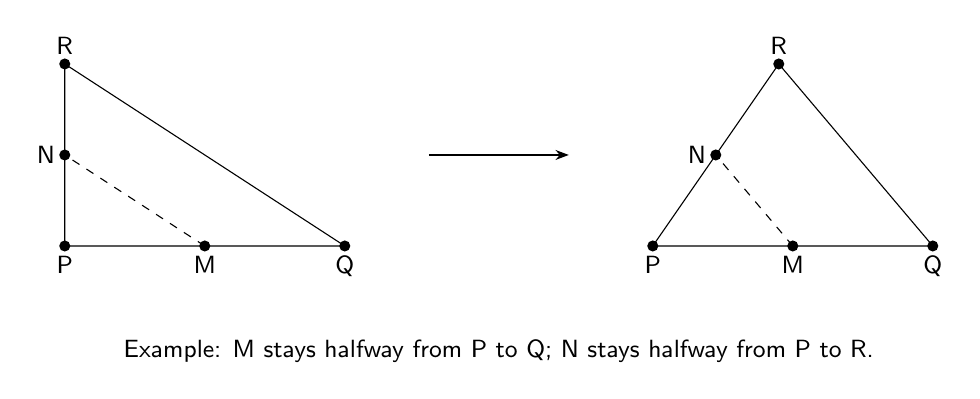
\begin{tikzpicture}[x=.7in,y=.7in,font=\small,>=Stealth]
\draw(0,0)--(2,0)--(0,1.3)--cycle;
\fill(0,0)circle(2pt)node[below]{P};\fill(2,0)circle(2pt)node[below]{Q};\fill(0,1.3)circle(2pt)node[above]{R};
\fill(1,0)circle(2pt)node[below]{M};\fill(0,.65)circle(2pt)node[left]{N};\draw[dashed](1,0)--(0,.65);
\draw[->](2.6,.65)--(3.6,.65);
\draw(4.2,0)--(6.2,0)--(5.1,1.3)--cycle;
\fill(4.2,0)circle(2pt)node[below]{P};\fill(6.2,0)circle(2pt)node[below]{Q};\fill(5.1,1.3)circle(2pt)node[above]{R};
\fill(5.2,0)circle(2pt)node[below]{M};\fill(4.65,.65)circle(2pt)node[left]{N};\draw[dashed](5.2,0)--(4.65,.65);
\node at(3.1,-.75){Example: M stays halfway from P to Q; N stays halfway from P to R.};
\end{tikzpicture}\end{center}
\fanboard
\vspace{.1in}
O's position: \hrulefill
\answerline\answerline\answerline
\newpage
\problem{3}{Make a rule that moves every point of the rectangle into the square, with no gaps, overlaps or tears. Each named side must land on the same named side. Keep every new distance at most twice its old distance. Draw where the dotted lines go. Your partner chooses two points anywhere and tests your rule.}
\begin{center}\begin{tikzpicture}[x=.94in,y=.94in,font=\small]
\draw[dotted,thick,step=.5] (0,.5) grid(4,1.5);\draw[thick](0,.5)rectangle(4,1.5);
\node at(2,.17){bottom: 4 units};\node at(2,1.8){top};\node[rotate=90]at(-.35,1){left: 1 unit};\node[rotate=90]at(4.32,1){right};
\begin{scope}[shift={(4.9,0)}]\draw[thick](0,0)rectangle(2,2);\node at(1,-.32){bottom: 2 units};\node at(1,2.3){top};\node[rotate=90]at(-.35,1){left};\node[rotate=90]at(2.35,1){right: 2 units};\end{scope}
\end{tikzpicture}\end{center}
My rule for every point:
\answerline\answerline
\vspace{.25in}
\problem{4}{Does your rule pass every possible pair, including points between the grid lines? Explain why. Could a different rule make every pair's stretch less than 2 while keeping the named sides?}
\answerline\answerline\answerline\answerline
\newpage
\problem{5}{Your partner chooses one of these new rectangles. Move the whole 4-by-1 sheet onto it, keeping the named sides. Find the smallest possible worst stretch. Give a rule for the whole sheet and find a pair that no legal rule can stretch less. Swap jobs for another rectangle.}
\begin{center}\begin{tikzpicture}[x=.6in,y=.6in,font=\small,>=Stealth]
\draw[thick](0,0)rectangle(4,1);\node at(2,-.38){4 by 1};\node at(2,1.3){top};\node[rotate=90]at(-.3,.5){left};
\draw[->](4.4,.5)--(5.1,.5);
\draw[thick](5.6,-.5)rectangle(11.6,1.5);\node at(8.6,-.88){6 by 2};\node at(8.6,1.8){top};\node[rotate=90]at(5.3,.5){left};
\end{tikzpicture}\end{center}
Smallest worst stretch: \rule{.7in}{.3pt}\quad Rule and unavoidable pair:
\answerline
\begin{center}\begin{tikzpicture}[x=.6in,y=.6in,font=\small,>=Stealth]
\draw[thick](0,0)rectangle(4,1);\node at(2,-.38){4 by 1};\node at(2,1.3){top};\node[rotate=90]at(-.3,.5){left};
\draw[->](4.4,.5)--(5.1,.5);
\draw[thick](6,-1)rectangle(8,2);\node at(7,-1.38){2 by 3};\node at(7,2.3){top};\node[rotate=90]at(5.7,.5){left};
\end{tikzpicture}\end{center}
Smallest worst stretch: \rule{.7in}{.3pt}\quad Rule and unavoidable pair:
\answerline
\vspace{.13in}
\problem{6}{Invent a new target rectangle whose smallest possible worst stretch is exactly $1\frac12$. Can your partner find a different one?}
\answerline\answerline
\end{document}
